\chapter{Code dans la carte principale}

\section{Mise en place de CCS}
\label{sec:MiseEnPlace}
\subsection{Installation de Code Composer Studio}
Afin de programmer correctement le DSP, une version spécifique de Code Composer Studio (CCS) ainsi qu'une bibliothèque dédiée au DSP doivent être installées.

La version requise de CCS est la suivante \cite{CCS_Install} :
\url{https://www.ti.com/tool/download/CCSTUDIO/12.6.0} \\

Pour la bibliothèque C2000Ware, la version suivante doit être installée \cite{C2000_Install} :
\url{https://www.ti.com/tool/download/C2000WARE/5.02.00.00}\\

\subsection{Configuration de CCS}

Une fois l'installation terminée, il est nécessaire de configurer CCS pour qu'il détecte la bibliothèque. La procédure d'intégration est la suivante :

\begin{enumerate}
    \item Lancer Code Composer Studio.

    \item Accéder au menu \textit{Window > Preferences}.

    \item Dans la colonne de gauche, naviguer vers \textit{Code Composer Studio > Products}.

    \item Vérifier la liste "Product discovery path". Si le dossier \verb|C:\ti| n'y figure pas, cliquer sur \textit{Add...} et le sélectionner.
    \item Cliquer sur le bouton \textit{Refresh}.

    \item La bibliothèque C2000Ware doit apparaître dans la liste « Discovered products ». Cliquer alors sur \textit{Install}.

    \item Si l'explorateur de fichiers s'ouvre, sélectionner l'emplacement exact du dossier (généralement \verb|C:\ti\c2000\C2000Ware_5_02_00_00|).

    \item Vérifier que le dossier est correctement coché et cliquer sur \textit{Apply and close}. La figure \ref{fig:Res_conf_C2000} illustre le résultat attendu.

          \begin{figure}[htbp]
              \centering
              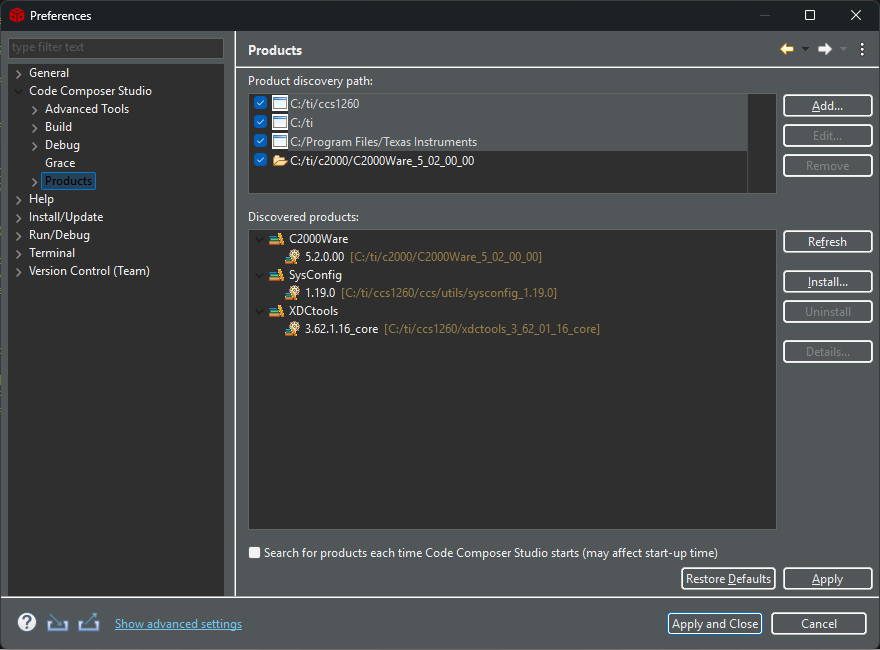
\includegraphics[width=0.75\linewidth]{Image/Chap.2/Resultat_conf_C2000.png}
              \caption{Résultat de la configuration du C2000}
              \label{fig:Res_conf_C2000}
          \end{figure}

    \item Une fois la configuration terminée, cliquer sur le bouton \textit{Build} pour appliquer les changements.
\end{enumerate}

Enfin, il est impératif de vérifier que le niveau d'optimisation de CCS est correctement établi en suivant ces étapes :

\begin{enumerate}
    \item Effectuer un clic droit sur le projet.

    \item Sélectionner \textit{Properties}.

    \item Dérouler l'onglet \textit{Build > C2000 Compiler > Optimization}.

    \item Appliquer les paramètres tels qu'illustrés dans la fenêtre suivante :

          \begin{figure}[H]
              \centering
              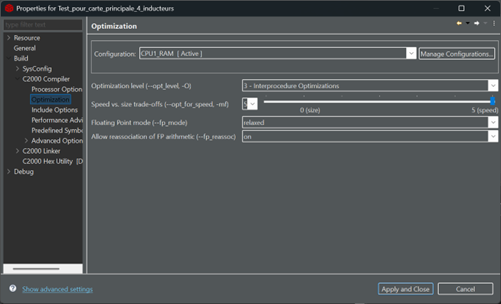
\includegraphics[width=0.75\linewidth]{Image/Chap.2/CCS_Opti_Windows.png}
              \caption{Configuration des paramètres d'optimisation}
              \label{fig:Res_conf_Opti}
          \end{figure}
\end{enumerate}

Lorsque le programme final est prêt, il faudra à ce moment-là flasher le code dans la mémoire flash afin que le code reste en "stand alone".

Il est désormais possible d'utiliser CCS pour la programmation du DSP.

\section{Code de départ}

\section{Amélioration du code}
